%===================================== CHAP 5 =================================

\chapter{Implementation}
To be able to answer the research questions using the methods described in the previous chapter, a system needed to be developed. This chapter covers the implementation and architecture of this system and its different components, including decisions on design, usability and development.

\section{System overview}

Utsida is a joint collaboration between two students with specializations in software and an artificial intelligence, respectively. This is reflected by a two-part system were each part primarily targets one of the research questions. Utsida was chosen as the name of the system due to being a counter opposite to NTNU's central system \emph{Innsida}, and the meaning of the word \emph{inside}. Utsida gives a relation to something on the outside, in this case going on an exchange program, including choosing a foreign university, and a set of courses at that university. As a whole, Utsida contains two sub-systems, where the first part is a CBRS, and the second part is a web application. The requirements identified in the preliminary research, see section \ref{sec:requirements}, was used as the basis for the design and implementation.

\begin{figure}[H]
    \centering
    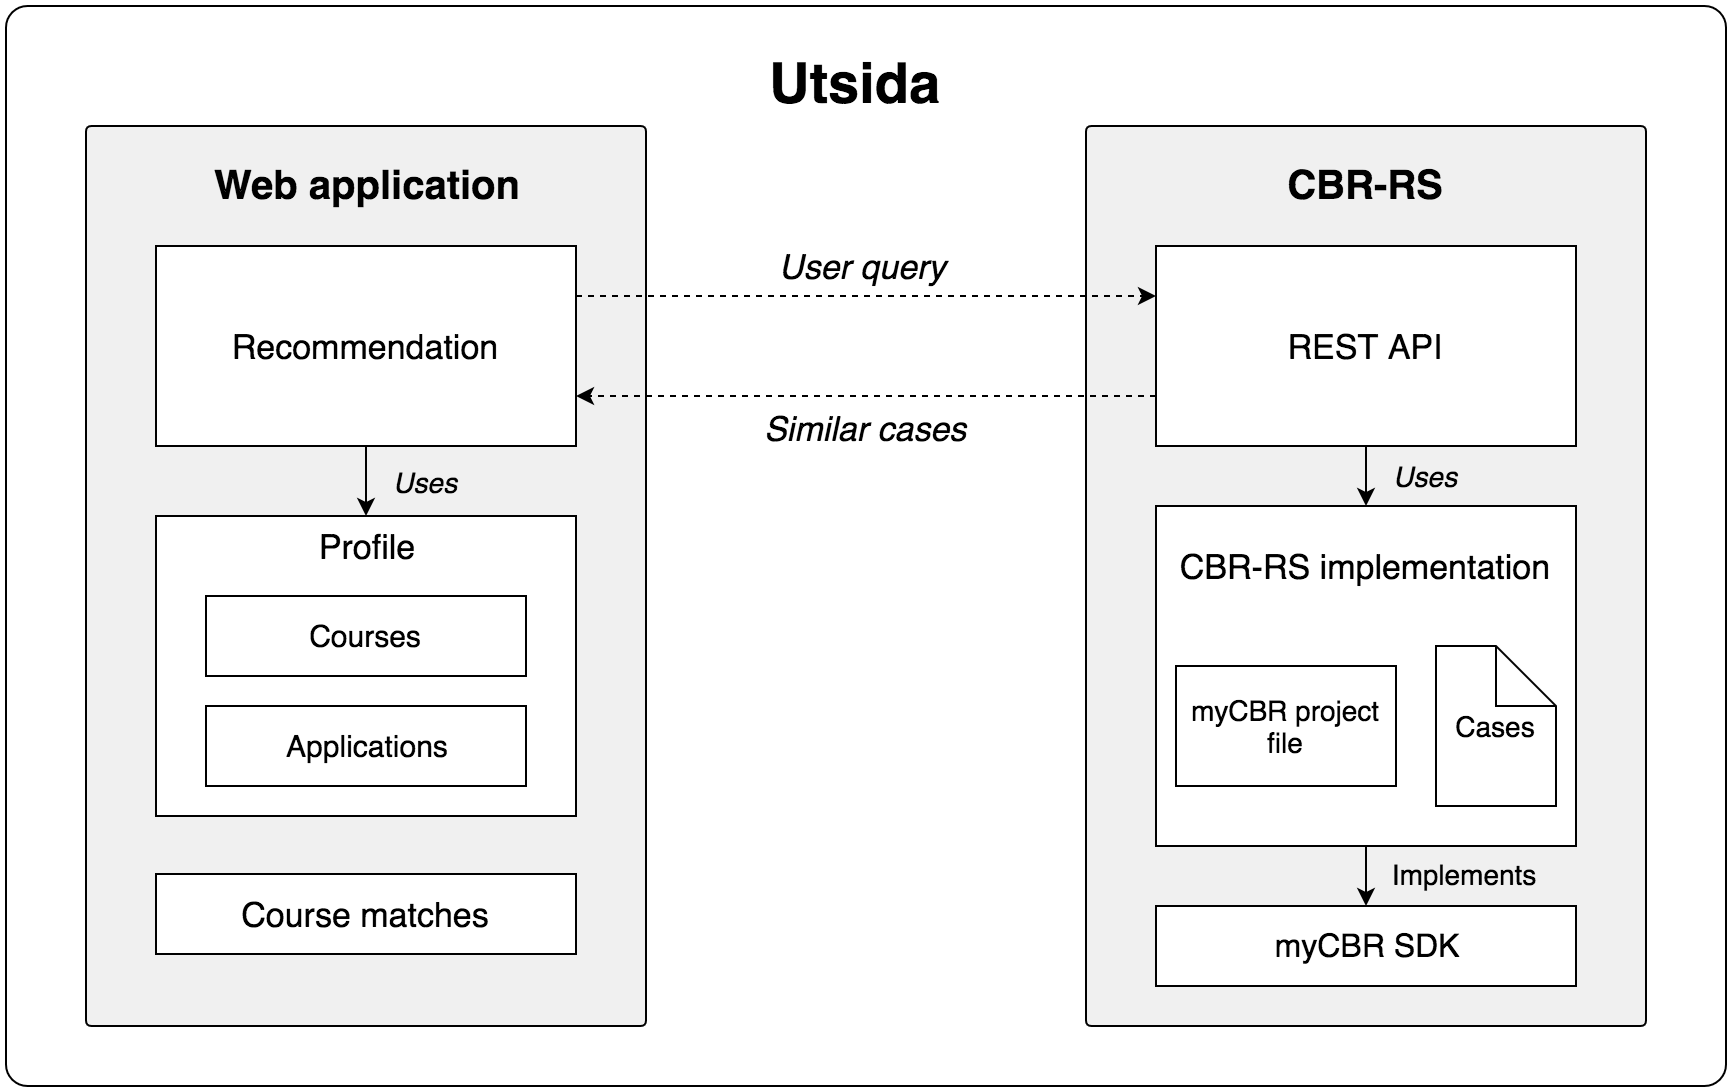
\includegraphics[width=1\textwidth]{fig/system_overview.png}
    \caption{Abstract architectural diagram of Utsida}
    \label{fig:system_overview}
\end{figure}


As illustrated by Figure \ref{fig:system_overview}, Utsida's web application part communicates with the CBRS part. Queries are sent from the web application by a user, and received by the CBRS through it's REST API. These queries are in turn matched against the entire case-base in the CBRS, and finally all the cases in the case-base are returned to the web application with a coherent similarity score with regards to the user query. Typically in a CBR system, the solution to a problem would be the solution of the case with the highest similarity score for the proposed problem. Utsida on the other hand, offers several possible solutions, because it is a case-based \textbf{recommender} system, rather than a case-based \textbf{reasoning} system. This way, the user can browse several solutions, and pick the one they want. 

The web application part of Utsida is divided into three main components, as figure \ref{fig:system_overview} depicts; \emph{Recommendations, Profile} and \emph{Course matches}. 

\subsection{Components of the Web Application}
The three main components of the web application contains all the functionality identified in the preliminary research as the system requirements (section \ref{sec:requirements}). The goal of the components as a whole is to answer RQ2 and to positively effect the motivation of students to go on an exchange program. 

\subsubsection{Recommendations}
This component is the part of the web application which communicates with the CBRS, by sending a query made by a user in JSON format to the CBRS through HTTP requests, which returns all of its cases with a coherent similarity score, also in JSON format. It serves as the core functionality of Utsida, and the tool to answer RQ1. A user can type in any information they like about what the wishes and requirements for their exchange study are, and are presented with a list of the best suiting universities for their query, followed by the best matching trips to each university which each contains a list of courses that were taken, and thus serves as the solutions, or recommendations.


\begin{figure}[h]
    \centering
    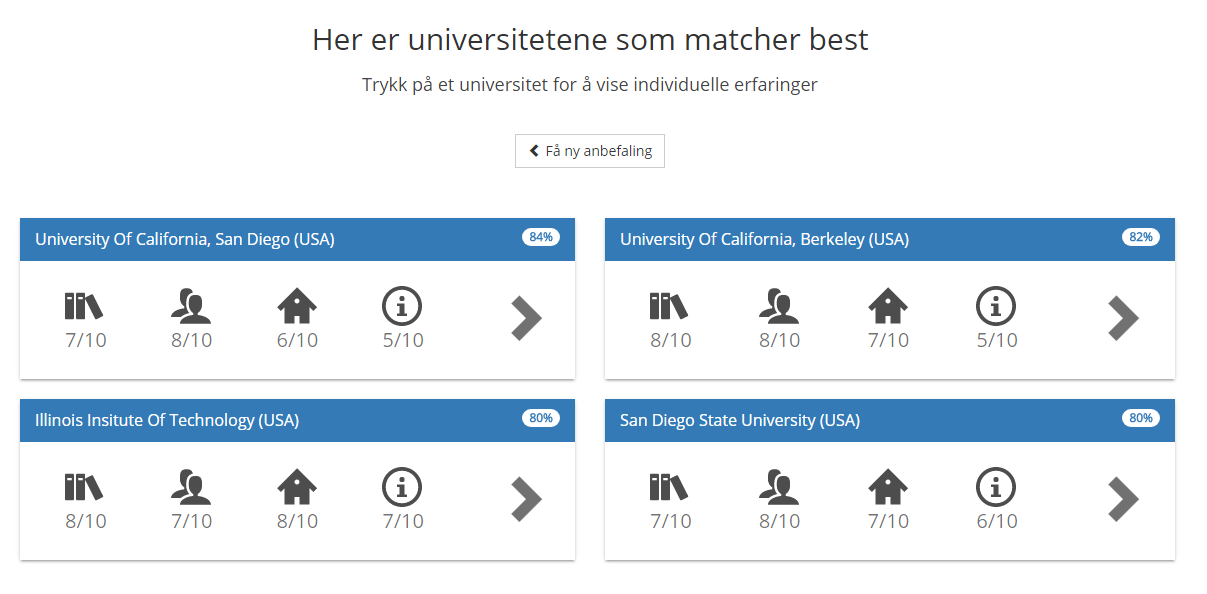
\includegraphics[width=1\textwidth]{fig/utsida_screenshots/results_1.PNG}
    \caption{How results are first presented after sending a query in Utsida}
    \label{fig:my_label}
\end{figure}

\begin{figure}[h]
    \centering
    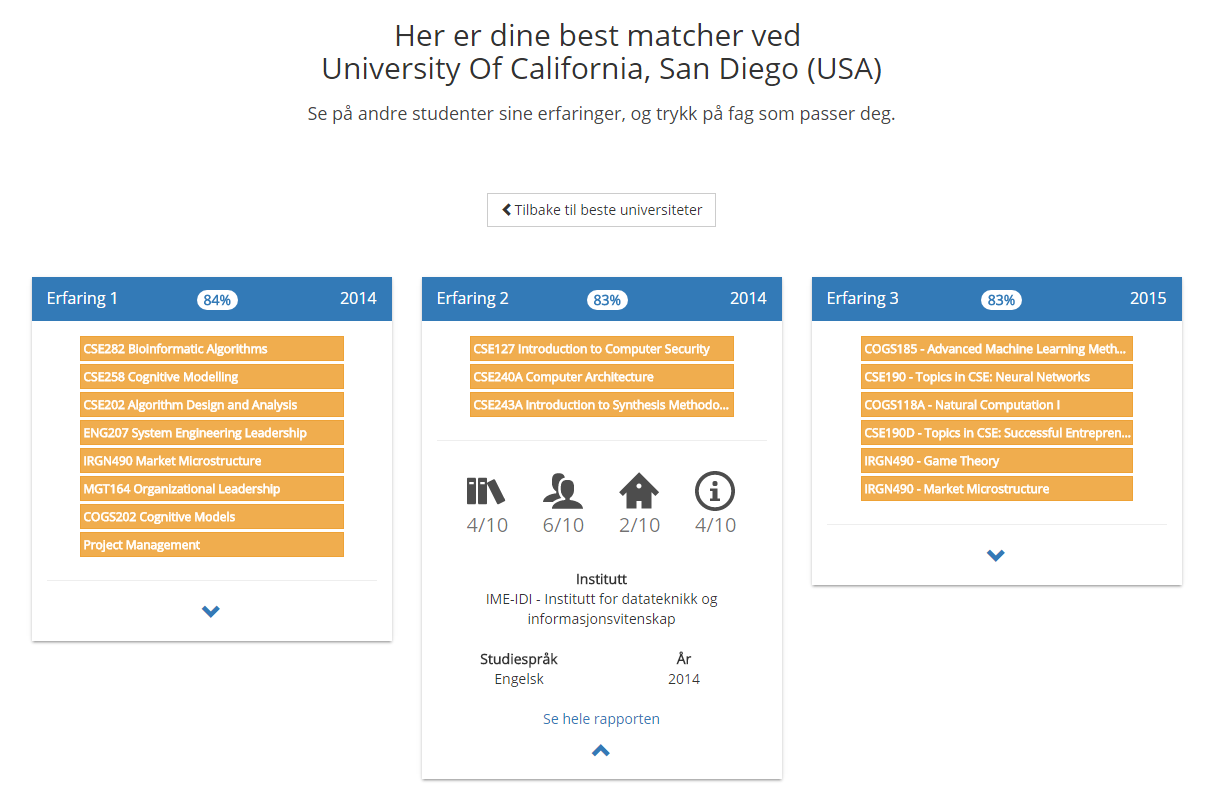
\includegraphics[width=1\textwidth]{fig/utsida_screenshots/results_2.PNG}
    \caption{How results are presented after selecting a recommended university in Utsida}
    \label{fig:my_label}
\end{figure}

\subsubsection{Course Matches}
The objective of the course matches component is to display all known approved course matches (sets of courses where one or more courses from another university are accepted as a replacement for a course at NTNU), ordered by universities. This component supports adding, deleting and editing course matches by student advisers, including comments. For a student, this component serves as a resource where they can search and find replacements for their courses based, and get information on both NTNU and abroad courses, approval data, which advisor who approved it, and finally save the course match to their profile. 

According to the survey send out by NTNU's International Section about the information students receive at NTNU with regards to going on study exchange programs in 2016, $85,34\%$ of 464 students stated that a list containing earlier approved course matches would increase the number of students going on study exchange programs. This functionality therefore felt essential to include. An issue however with this component proved to be that gathering information about these earlier approved course matches was hard, and it was cumbersome to convert them all to the same format to fit Utsida. Therefore, an initial list was created in Utsida, with the intention that student advisers could expand on this lit in the future.

\begin{figure}[h]
    \centering
    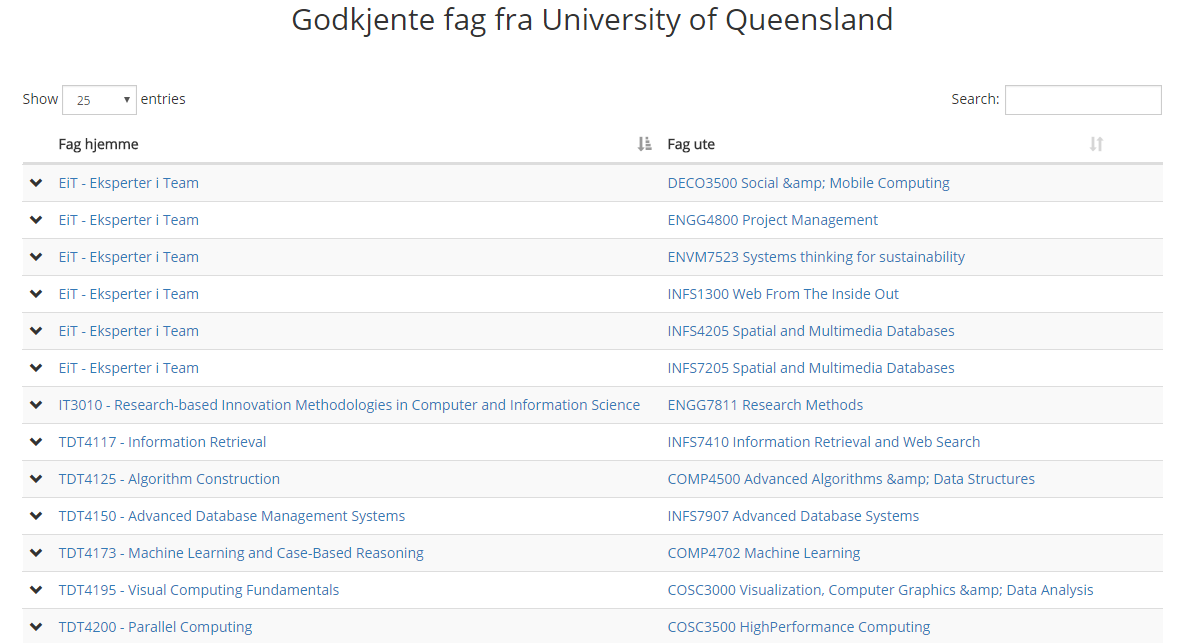
\includegraphics[width=1\textwidth]{fig/utsida_screenshots/approved_courses.PNG}
    \caption{Sample list from Utsida's approved course matches page}
    \label{fig:my_label}
\end{figure}

\subsubsection{Profile}

The profile component handles all user related functionality, such as authentication, and contains the required personal information about each student. This information includes their current institute at NTNU, which is used in a recommendation query. It is one of the greatest attributes to match against other students' exchange study experiences, because it indicates that their courses should be at least somewhat similar. Furthermore, it includes the following sub-components.

\paragraph{Courses} is a sub-component of the profile component. It contains many useful functionalities students can use to organize their application process, such as storing courses they find through Utsida's recommendation component, course matches they find in the course matches component, courses they need to replace at NTNU, and all of their course matches. From the course page, students can also manually match abroad- and home courses to create new course matches for their applications. This component serves as a large part of the whole application chain, and is needed to digitalize it. 

\begin{figure}[h]
    \centering
    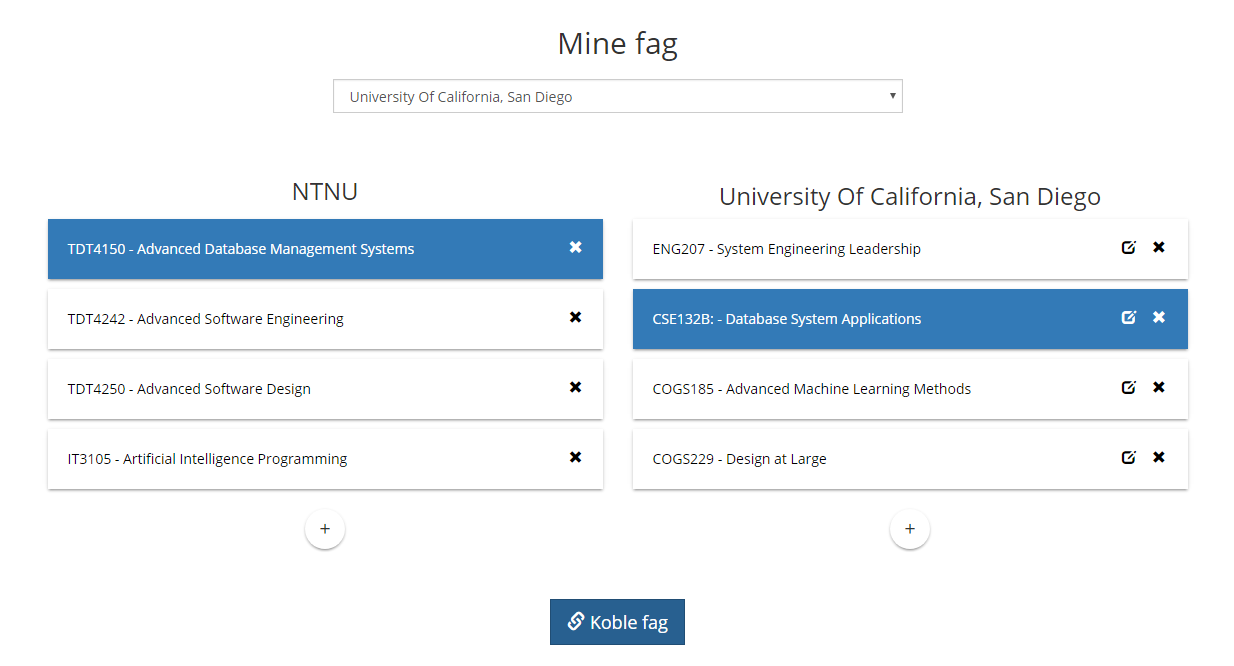
\includegraphics[width=1\textwidth]{fig/utsida_screenshots/course_match.png}
    \caption{The view for saving, viewing and matching courses in Utsida.}
    \label{fig:my_label}
\end{figure}

\paragraph{Applications} is also a sub-component of the profile component. It stores all applications the user has committed, meaning all the course matches the user has applied to get approved by a student advisor. Furthermore, it maintains the functionality needed to create applications. For students and student advisers, the application component serves as a digital version of the current paper based application system where student advisers can approve, reject, and remove students' application, while students can easily keep track of them. This component is an extension needed to complete Utsida as a functional and usable replacement.

\begin{figure}[H]
    \centering
    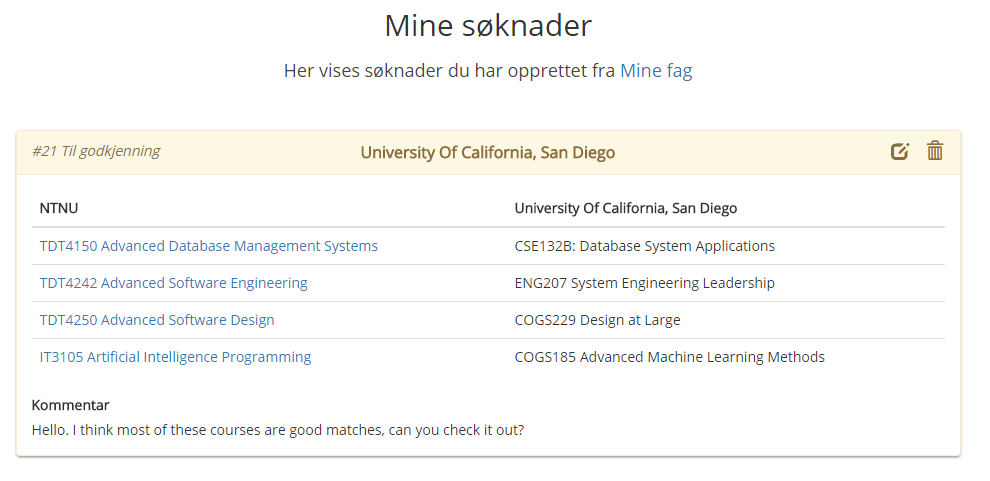
\includegraphics[width=1\textwidth]{fig/utsida_screenshots/application_list.PNG}
    \caption{The view showing a user's active applications in Utsida}
    \label{fig:my_label}
\end{figure}

\section{Data and Information used in Utsida}
Utsida requires up to date organizational data about NTNU to be usable. This includes:

\begin{itemize}
    \item Courses at NTNU: All current courses possible to take at NTNU are added to Utsida's database so that students can pick the courses they need in the web application.
    \item Faculties and institutes at NTNU: To complete a profile in the web application, a student has to pick their institute, so that it can be used as an attribute when querying the CBRS, therefore all possible institutes at NTNU are added to Utsida's database.
\end{itemize}

This data was gathered with IDI's organization API for NTNU\footnote{http://www.ime.ntnu.no/api/}, which unfortunately recently was discontinued, so to update this data, a new data source would have to be found. 

Furthermore, the course matches component in the web application relies on information on previous approved course matches, which is logged by some student advisers at NTNU. Obtaining this data presented several difficulties, because there are no standard way to keep track of these approvals at NTNU. Thus, only approved course matches for departments which we found were added (mostly IDI). Furthermore, the entries which was obtainable were in different formats, which required an extensive parser script to transform and add to Utsida's database.

The most important data however, was the data needed to create cases in the CBRS' case-base, namely The Office of International Relations' \textit{experience reports}.

\subsection{The Experience Reports}\label{sec:experience_reports}
Typically, a CBRS' case-base is gradually expanded as new cases are retained. In this project, it was essential to have a large number of cases in the case-base from the start. A large part of the motivation for doing this research stems from personal experience, and thus the current process for applying for a study exchange program at NTNU was well known. Most students who go on an exchange program at NTNU has to write obligatory reports to The Office of International Relations at NTNU. These reports are available to the public, and because of all the information about an exchange study they include, they proved to work as a great base for a case. All of the current public experience reports were downloaded and parsed (see section \ref{sec:parsing_experience_reports}) to cases, and then added to the CBRS' case-base. With this in place, the data and foundation of the CBRS was in place.

\subsection{Parsing the Experience Reports}\label{sec:parsing_experience_reports}
The experience reports are essentially large text files in HTML format. To be able to use them in Utsida, all the useful information in the HTML files had to be extracted and finally be converted to entries in a large CSV file, which is the file type MyCBR use as a case-base. A quite extensive python script was written to handle this.

In short, all available experience reports (HTML files) were first downloaded and stored in a directory. The script then loops through all of the HTML files, reads the data with the use of the python package \emph{HTMLParser}\footnote{https://docs.python.org/2/library/htmlparser.html}, saves all the useful data in a dictionary which is converted to one row in the CSV file which serves as the case-base. This way, each row in the CSV file corresponded to one case with the attributes given by table \ref{tab:case_representation2}. This finally resulted in a case-base with 8702 cases.

The job of parsing these files turned out to be extremely time consuming affair because most of the information in the files consisted of free text. This implies that the writers of each report decided themselves how to write the university they went to, the courses they took, their department and the rest of the information which was vital for the cases. To handle this, the script has one method to format each attribute to the correct format in terms of Utsida. Beside writing string handling for all kinds of edge cases in python, there were two noteworthy techniques used; data dictionary look-ups and approximate string matching (fuzzy searching).


\paragraph{Fuzzy Searching}
Fuzzy Searching is an algorithm used to recognize patterns and similarities in text, and yield a score to determine the similarity between them. Using this technique in the script which parsed the experience reports, predefined sets of attributes could be formatted as the system required, for then to use fuzzy search on the text input in the reports to map the most similar occurrences to predefined data. For example, in the field in the reports where the students wrote their department at NTNU, a huge variation of abbreviations, and differentiation in ways of spelling the department was an issue. By creating a dictionary with all departments and faculties, fuzzy searching could be used to match the input in the report to this dictionary, and return the record in the dictionary with the highest similarity score to the input in the report. This method was also used to avoid creating multiple instances of the same university in the database, because they were written slightly different. Data dictionaries were created in python for countries, continents, languages, universities, departments and faculties to be able to map the important data in the experience reports to a correct format.

\begin{figure}[h]
    \centering
    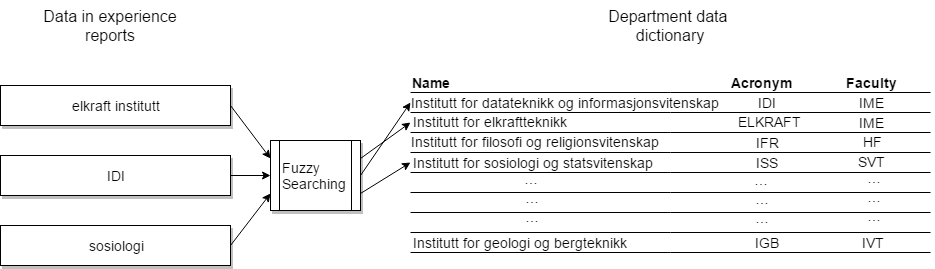
\includegraphics[width=1.0\textwidth]{fig/fuzzy_search.png}
    \caption{Input data is transformed to a set format by using fuzzy searching}
    \label{fig:fuzzy_searching}
\end{figure}

In the end, most of the data in the experience reports was transformed to usable data in the CBRS. However, making sure all the data stemming from user input in all of the 8702 experience reports was represented in a correct way in the CBRS, as well as being meaningful was not realistic nor possible. 

\subsection{Data Quality Evaluation}
Cleaning and validating the data in both the digital course match tables written by student advisers, and the experience reports was an important step to perform before any of it was parsed. The data is analyzed according to the six primary dimensions for data quality assessment\cite{askham2013six} in the following paragraphs.

\paragraph{Completeness} indicates the percentage of stored data versus the total amount of data, which in this case are all the experience reports. Utsida's case-base consists of 8702 cases. However, on The Office of International Relations' website for experience reports, the index goes up to 17012. It is unknown how many reports which are actually published on this site, because a large amount of these indexes doesn't point to an experience report, hence, there are a lot less than 17012. Furthermore, many reports were preliminary excluded if they were missing vital information such as which department the student belonged to, or which courses they took on the trip. Without either of this data, a case doesn't give much value to the system. In the end, the cases in the case-base does not represent 100\% completeness with regards to all available experience reports, but they include most of them.

\paragraph{Uniqueness} represents the percentage of data entries which are unique. There is no control regarding eventual duplicate cases in the case-base. Since each case is an individual experience, they are considered unique all though two or more students may have chosen the exact same geographical place, university, and courses. However, the probability for two cases to be identical is quite slim, as there are so many different attributes and values. Furthermore, in this project, multiple similar cases- even identical ones only strengthen the recommendations for a given query. Other data, such as the assessed course matches, both abroad- and home courses etc. are required to be unique in Utsida's database, and thus yields a uniqueness of 100\%.

\paragraph{Timeliness} is the degree to which data represent reality from the required point in time \cite{askham2013six}. The last experience report in the data set was published in 2016, while the first one was published in 1999. The data set should include entries from 2017, but the system for submitting experience reports underwent some changes and updates during fall 2016, and was therefore frozen until spring 2017. This means the newest data in the case-base is already 1 year older than the current year during the writing of this report (2017). The experience reports tend to be submitted either a couple of months after an exchange period, or in the middle of one. This makes the timeliness have a great degree of variation and is difficult to assess. However, even if a student's experience is 3 years old, it is still likely to be very relevant. Furthermore, the study period attribute is handled in the CBRS by reducing a reports relevancy the older it is.

\paragraph{Validity} considers the validity of data, which is valid if it conforms to the syntax (format, type, range) of its definition \cite{askham2013six}. Most of the data in the experience reports were not validated in any way; they accepted free text. Because they had no range or constraint, there had to be done exceptionally much validation of data in the script which parsed these reports into cases. The same goes for the assessed course matches.

\paragraph{Accuracy} is the degree to which data correctly describes the \enquote{real world} object or event being described \cite{askham2013six}. Both the data in the experience reports and the assessed course matches is mostly free text, and thus it is hard to measure it's accuracy properly. There are no set bounds, ranges and constraints for much of the data, meaning it simply have to be interpreted. As described in section \ref{sec:parsing_experience_reports}, measures were made to convert data from their free text form to a given format in Utsida, but there are no guarantees for the data ending up as the original user intended.

\paragraph{Consistency} is described as the absence of difference, when comparing two or more representations of a thing against a definition \cite{askham2013six}. In the experience reports, this property is considered high. Each report is written in the same exact format, with the same descriptions and values. The assessed course matches however lack consistency because the format they are written in depends on the student adviser who wrote them, making them require some analysis and pre-processing before being usable. 

Conclusively, the largest data resource used in this project, the experience reports, is considered to measure poorly in some of the six primary dimensions for data quality assessment. Extensive pre-processing and analysis of the data, was essential. All though the methods used may overlook some invalid or bad data, it is considered too small to influence the CBRS' recommendations in a noticeable way. 


\section{The CBRS Model}
This section describes how to CBRS' model was implemented and how the system was developed. This includes how its cases are represented, which taxonomies and similarity measures are used, how the weighting of the attributes in a case was done, and how the system itself was implemented.

\subsection{Case Representation in Utsida}

When parsing the experience reports, choices had to be made in regards to what data was needed. One of the most important aspects of Utsida, is that it should be fast and simple to use. Therefore, the amount of attributes and data extracted from the reports were initially narrowed down to a minimum, but still chose the data which yielded the most importance. The initial chosen data and attributes were modelled to the key-value pairs in Table \ref{tab:case_representation1}.


\begin{table}[H]
\centering
\small
\caption{Initial representation of a case in Utsida}
\label{tab:case_representation1}
\begin{tabulary}{\textwidth}{|L|L|}
\hline
\textbf{Attributes} & \textbf{Example Case} \\ \hline
Home Institute & IME-IDI - Institutt for datateknikk og informasjonsvitenskap \\ \hline
Destination Continent & North America \\ \hline
Destination Country & USA \\ \hline
Destination University & UCLA \\ \hline
Study Language & English \\ \hline
Study Period & 2012 \\ \hline
Academic Quality Rating & 4 \\ \hline
Social Quality Rating & 2 \\ \hline 
Subjects Taken & \begin{tabular}[c]{@{}l@{}}COMP1927 - Computing 2\\ MATH3220\\ CS4210\\ DATA101\end{tabular} \\ \hline
\end{tabulary}
\end{table}

This representation was used during the first usability test phase. From the feedback and interviews in the tests, new information and ideas about good attributes to include was acquired, such as ease of finding a place to live, the standard of said place, the amount of support the students received at their chosen university, and the general cost of living in the country. These results combined with the groups identified from a paper on important international student factors \cite{maria2006international} lead to a an extended case representation, which is displayed in Table \ref{tab:case_representation2}. This revision also spliced several ratings which was significant for the social aspects into the social quality rating, and the same for the academic.

\begin{table}[H]
\centering
\small
\caption{Extended representation of a case in Utsida}
\label{tab:case_representation2}
\begin{tabulary}{\textwidth}{|L|L|}
\hline
\textbf{Attributes} & \textbf{Example Case} \\ \hline
Home Institute & IME-IDI - Institutt for datateknikk og informasjonsvitenskap \\ \hline
Destination Continent & North America \\ \hline
Destination Country & USA \\ \hline
Destination University & UCLA \\ \hline
Study Language & English \\ \hline
Study Period & 2012 \\ \hline
Academic Quality Rating & 8 \\ \hline
Social Quality Rating & 4 \\ \hline
Ease to find- and quality of residential & 5 \\ \hline
Support and reception at university & 6 \\ \hline
Subjects Taken & \begin{tabular}[c]{@{}l@{}}COMP1927 - Computing 2\\ MATH3220\\ CS4210\\ DATA101\end{tabular} \\ \hline
\end{tabulary}
\end{table}

To finalize the case model, and also to form a basis for how important each of these attributes should be in a query, a questionnaire was sent out to a selected group of students (see Chapter \ref{chap:4}, section \ref{sec:questionnaires}).

\subsubsection{The Problem Part}

The following list elaborates the choice and significance of the different attributes used in a case.

\begin{itemize}
\item \textbf{Home Institute:} The home institute is considered the most important attribute, as it contains information about the student's faculty and institute at home, as well as a pointer to what kind of courses which are relevant to the student. This was quantified during the initial usability testing of the system; even though the geographical location and university, as well as every other factor seemed like a perfect fit, the suggestion is not valid if the suggested courses are irrelevant for the user. 

\item \textbf{Destination Continent:} The continent is included both to give the user the opportunity to filter countries based on a continent, and to be able to only choose a continent if they are unsure of which country they would like to go to. 

\item \textbf{Destination Country:} The country serves as the most specific geographical option.

\item \textbf{Destination University:} The university is included to match exact universities in a case, if the user knows exactly which university they would go to.

\item \textbf{Study Language:} The study language represents they language which was reportedly used in a case. 

\item \textbf{Study Period:} The study period is included to make older cases less relevant to the user, as a university's infrastructure often changes over time. The option is hidden, and thus not selectable to the user. This way, any query will automatically send the current year. 

\item \textbf{Academic Quality Rating:} A rating which is a conjunction of an experience report's \emph{Academic Quality}, \emph{Special Competence Gained} and general \emph{Quality of Academic Opportunities}. Each of these aspects are related to the academic quality of an experience, and are weighted differently.

\item \textbf{Social Quality Rating:} A rating which is a conjunction of an experience report's rating of  \emph{Social Quality}, \emph{Leisure Activities}, \emph{Girlfriend/friends}, the social interaction with \emph{Students from the University}, \emph{Other Foregin Students} and \emph{Norwegian Students}. Each of these aspects are related to the social quality of an experience, and are weighted differently.

\item \textbf{Ease to find- and Quality of Residential:} A rating which is a conjunction of an experience report's rating of \emph{Residential Dissemination} and \emph{Residential Quality}. Each of these aspects are related to the residential part of an experience, and are weighted differently.

\item \textbf{Support and Reception at University:} A rating which is a conjunction of an experience report's rating of \emph{General Reception} and \emph{Administrative Support}. Each of these aspects are related to the support a student received at the university in an experience, and are weighted differently.
\end{itemize}

It is important to note that a query in Utsida is feasible with any number of selected attributes, the more attributes which are selected, the more relevant the results will be. 


\subsubsection{The Solution Part}
The solution to each case is the subjects the student chose. Considering another struggle for students wanting to apply for a study abroad- or study exchange program is to chose an university as well, the chosen university can also be viewed as a part of the solution to the case. With the mentioned attributes in place, the solution (the chosen subjects) should be relevant for the student, while the location should be feasible. 

\subsection{Taxonomies}\label{sec:taxonomies}
According to Michael M. Richter \& Rosina O. Weber\cite{richter2013case}, taxonomies are widely used structures and specialisations of graphs. They relate
objects to each other. The intention is to do this in a hierarchical way, going from
general to more specific objects. This implies that branching leads to objects that
have more in common. 

In Utsida's CBR model, several attributes are a perfect fit for using a taxonomy to organize objects directly. For example, if a query contains a country, instead of only yielding a similarity score on how good this country matches with the country in each case, it will also yield a given similarity score if the country resided within the same continent as the country in the query. Figure \ref{fig:country_taxonomy} illustrates how the taxonomy for a country's similarity score is modelled in Utsida.

\begin{figure}[H]
    \centering
    \includegraphics[width=0.8\textwidth]{fig/country_taxonomy.png}
    \caption{Brief illustration of the taxonomy for the country attribute}
    \label{fig:country_taxonomy}
\end{figure}

If the country in a query is an exact match with the country in a case, the similarity score for the country attribute in that case will be 1.0. If it is a different country, but it still resides within the same continent as the country in a case, it will yield a similarity score of 0.3. No match at all will yield a 0.0. The same taxonomy is in place for the \emph{Home Institute} attribute, albeit ordered under the different faculties instead. Thus the faculty also works as a hidden attribute. The shared similarity for countries residing in the same continent differs on each continent, as some continents have less similarity between its countries than others. Specifically, the similarities in the taxonomy for the country attribute is as shown in Table \ref{tab:continent_similarity}, while the similarities in the taxonomy for the institute attribute are equally set to 0.3.

\begin{table}[h]
\centering
\caption{Taxonomic similarity of each continent}
\label{tab:continent_similarity}
\begin{tabulary}{\textwidth}{|L|L|}
\hline
\textbf{Continent} & \textbf{Similarity} \\ \hline
North America & 0.2 \\ \hline
South America & 0.3 \\ \hline
Oceania & 0.4 \\ \hline
Asia & 0.3 \\ \hline
Europe & 0.2 \\ \hline
Africa & 0.4 \\ \hline
\end{tabulary}
\end{table}

\subsection{Attribute Similarity Measures}
Each attribute in the case-model was assigned a designated similarity measure in addition to the taxonomies, which essentially are functions returning a similarity score based on the similarity between the attribute in a query, and the coherent attribute in a case. Following, each of these measures are detailed and explained.

\begin{itemize}
    \item \textbf{Rating Similarity:} In the case-model, the attributes \emph{AcademicQuality}, \emph{SocialQuality}, \emph{ReceptionQuality} and \emph{ResidentialQuality} are conjunctions of different ratings given in the experience reports. Each rating ranges between 1-10, and reflects how the student experienced their trip with regard to these categories. To calculate the similarity between a rating in a case, and a rating from a query, the CBRS uses Symmetric Difference Determined Similarity\cite{bergmann2002experience} with a linear function. It describes the decrease in similarity depending on the increase of the difference at a linear phase.
    
$\begin{displaystyle}
    f(d) = 
    \begin{cases} 1 : & d < min \\ 
    \frac{max-d}{max-min} : & min \leq d \leq max \\
    0 : & d > max
    \end{cases}
\end{displaystyle}$

    \item \textbf{Continent Similarity:} The continent attribute is a \emph{Symbol type}, meaning its allowed values are a pre-determined set. Similarity between continents are calculated with a $m x n$ matrix, where each mapping yields a given similarity, as displayed in table \ref{tab:continent_similarity}. The values are rough estimates with regards to similarity in culture, language, location and general university structure.

    \begin{table}[H]
    \small
    \centering
    \caption{The $m x n$ matrix for calculating similarity between continents}
    \label{tab:continent_similarity}
    \begin{tabular}{|
    >{\columncolor[HTML]{C0C0C0}}l |
    >{\columncolor[HTML]{FFFFFF}}r |
    >{\columncolor[HTML]{FFFFFF}}r |
    >{\columncolor[HTML]{FFFFFF}}r |
    >{\columncolor[HTML]{FFFFFF}}r |
    >{\columncolor[HTML]{FFFFFF}}r |
    >{\columncolor[HTML]{FFFFFF}}r |}
    \hline
    Attribute value & \cellcolor[HTML]{C0C0C0}South America & \cellcolor[HTML]{C0C0C0}Asia & \cellcolor[HTML]{C0C0C0}Europe & \cellcolor[HTML]{C0C0C0}Africa & \cellcolor[HTML]{C0C0C0}North America & \cellcolor[HTML]{C0C0C0}Oceania \\ \hline
    South America & 1.0 & 0.0 & 0.2 & 0.0 & 0.3 & 0.0 \\ \hline
    Asia & 0.0 & 1.0 & 0.0 & 0.0 & 0.0 & 0.0 \\ \hline
    Europe & 0.2 & 0.0 & 1.0 & 0.0 & 0.2 & 0.2 \\ \hline
    Africa & 0.0 & 0.0 & 0.0 & 1.0 & 0.0 & 0.0 \\ \hline
    North America & 0.3 & 0.0 & 0.2 & 0.0 & 1.0 & 0.2 \\ \hline
    Oceania & 0.0 & 0.0.0 & 0.2 & 0.0 & 0.2 & 1.0 \\ \hline
    \end{tabular}
    \end{table}
    
    \item \textbf{Country and Institute Similarity:} In addition to using the taxonomy described in section \ref{sec:taxonomies}, both the country- and institute attributes are matched directly between the the query and a case. The attributes are \emph{Symbol} types, and thus yields a similarity score based on the similarity between the two strings.
    
    \item \textbf{Language Similarity:} In the experience reports, the language field promoted a free-text answer. To handle this, the experience report parser created a list of all languages mentioned in this answer, and added it to the case. Thus, the Language attribute in a case is a list of strings. The attribute is represented as a \emph{Symbol} type which allows multiple values, such as a list. The function used to calculate the similarity between a query attribute and a case attribute simply yields a similarity of $1.0$ if it is an exact match (for example if a query contains the Language attribute \emph{Spanish}, and a case has the same in its Language field). If such a query was matched with a case with the list of the languages \emph{English, Spanish}, it returns the mean similarity for each item in the list. In this case, it would return a similarity of $0.5$, because it simply yields a $1.0$ for \emph{Spanish} and $0.0$ for \emph{English}.
    
    \item \textbf{University Similarity:} The university attribute is a simply string type. The similarity measure for calculating the similarity between two universities thus simply returns 1.0 if they are a complete match, or 0.0 if they differ in some way. All though it would be desirable to yield partly similarity if two strings are somewhat similar, it is limited by the string type in MyCBR, and it would not be possible to represent this attribute as a symbol type, because there is no way to pre-define each and every university which may occur in the system. 
    
    \item \textbf{Study Period Similarity:} The similarity measure used for the study period attribute is defined by a declining graph, where the similarity score decrease according to the distance in years between the query and a case. The points are plotted manually and is designed to greatly decrease the similarity score when a case is older than 5 years. Figure \ref{fig:study_period_graph} illustrates the graph.
    
    \begin{figure}[H]
        \centering
        \caption{The decline of similarity score according to the distance in years between a query and a case.}
        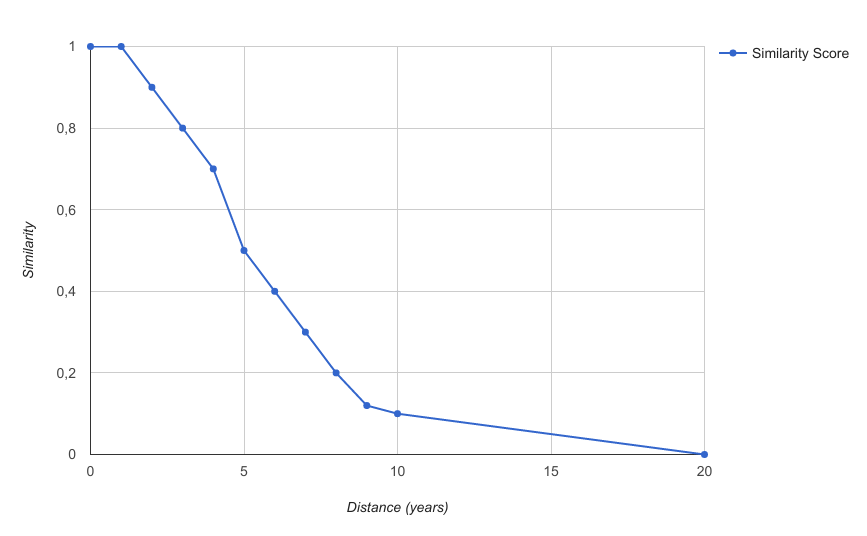
\includegraphics[width=1.0\textwidth]{fig/study_period_graph.png}
        \label{fig:study_period_graph}
    \end{figure}
    
\end{itemize}

\subsection{Sum Functions}
Before giving each case in the case-base a similarity score based on a query, the result of the similarity measure on each attribute is summarized, with regards to the attribute's weight. These functions are called Multi-Criteria Decision Making Methods (MCDMM).

There are two sum functions in the MyCBR Workbench, namely the Weighted Sum Model (WSM) and the Euclidean Distance (ED). For single dimensional problems (such as in this system), the WSM can be used without difficulties, and is probably the most common approach \cite{triantaphyllou2000multi}, and is given by the following expression \cite{fishburn1967letter}

\begin{displaymath}
    A^{*}_{WSM-score}\quad =\quad max_{i}\  \sum\limits_{j = 1}^{n}\  a_{ij}w_{j},\quad for \quad i =1,\ 2,\ 3,\ ...,\ m.
\end{displaymath}

When the CBRS receives a query from Utsida, a decision matrix is calculated for each case. This is a $(m \times n)$ matrix where each row is the attribute values of a case, paired with that attributes weight. 


\begin{table}[h]
\centering
\caption{A typical decision matrix for a query from Utsida to the CBRS}
\label{tab:decision_matrix}
\begin{tabular}{lllcccl}
                      &                       &                       & \multicolumn{1}{l}{} & \multicolumn{1}{l}{} & \multicolumn{1}{l}{} &                       \\
Attribute             & $Country$             & $Language$            & \ldots               & \ldots               & \ldots               & $AcademicQuality$     \\\hline
Weight                & $w_{country}$         & $w_{language}$        & \ldots               & \ldots               & \ldots               & $w_{country}$         \\\hline
$case_{1}$            & $sim_{case_{1}}$      & $sim_{case_{1}}$      & \ldots               & \ldots               & \ldots               & $sim_{case_{1}}$      \\
$case_{2}$            & $sim_{case_{2}}$      & $sim_{case_{2}}$      & \ldots               & \ldots               & \ldots               & $sim_{case_{2}}$      \\
\multicolumn{1}{c}{.} & \multicolumn{1}{c}{.} & \multicolumn{1}{c}{.} & \ldots               & \ldots               & \ldots               & \multicolumn{1}{c}{.} \\
\multicolumn{1}{c}{.} & \multicolumn{1}{c}{.} & \multicolumn{1}{c}{.} & \ldots               & \ldots               & \ldots               & \multicolumn{1}{c}{.} \\
\multicolumn{1}{c}{.} & \multicolumn{1}{c}{.} & \multicolumn{1}{c}{.} & \ldots               & \ldots               & \ldots               & \multicolumn{1}{c}{.} \\
$case_{m}$            & $sim_{case_{m}}$      & $sim_{case_{m}}$      & \ldots               & \ldots               & \ldots               & $sim_{case_{m}}$     
\end{tabular}
\end{table}

The WSM is used on this matrix to finally give each case in the case-base a similarity score between $0-1.0$, with regards to the query which the CBRS received. The CBRS then returns the list of the most relevant cases back to Utsida, which handles the rest.


\subsection{Weighting the Attributes}\label{sec:weighting}

Each attribute in a case has a value, and an associated weight. This is essentially just an integer denoting the importance of that attribute. During the modelling of the MyCBR project, these weights were chosen by the authors based on personal experience. These weights were in place during the usability testing, to learn if they seemed appropriate or not. To get a more public agreed upon set of weights, a questionnaire (see section \ref{sec:questionnaire_1}) was sent out to a set of relevant student where they were asked to give their opinion of what kind of attributes were the most important when selecting location and courses for an exchange study, and specifically how important each of these attributes were. 

Based on the Coefficient of Variance from table \ref{tab:attribute_ranking}, which takes both the mean and standard deviation in consideration, the attributes in the CBR model was configured as table \ref{tab:attribute_weights} shows.

\begin{table}[h]
\centering
\caption{Finalized weighting of the case attributes}
\label{tab:attribute_weights}
\begin{tabulary}{\textwidth}{LR}
\textbf{Attribute} & \textbf{Weight} \\ \hline
Home Institute & 7.0 \\ \hline
Destination Continent & 2.5 \\ \hline
Destination Country & 4.0 \\ \hline
Destination University & 4.0 \\ \hline
Study Language & 4.0 \\ \hline
Study period & 4.5 \\ \hline
Academic Quality Rating & 3.0 \\ \hline
Social Quality Rating & 3.0 \\ \hline
Ease to find- and quality of residential & 1.5 \\ \hline
Support and reception at university & 2.5
\end{tabulary}
\end{table}



\subsection{Implementation}

Since the MyCBR SDK requires a Java environment, an initial problem was how to couple this functionality with a web application. Luckily, Kerstin Bach, researcher at the Department of Computer and Information Science, NTNU is a contributor to the MyCBR project, and implemented the basis for a REST (Representational State Transfer) framework for a running MyCBR application. The CBR part of the system could then be a separate module, communicating with Utsida's web application only with HTTP requests.

The CBRS was first modelled using the MyCBR Workbench. This includes to create all the desired attributes shown in table \ref{tab:case_representation2}, selecting their types and restraints, and creating a similarity measure or taxonomy for each of them. The function for calculating a case's final similarity to a query is chosen, and each similarity measure is properly weighted.

\begin{figure}[H]
    \label{fig:workbench_exmaple}
    \centering
    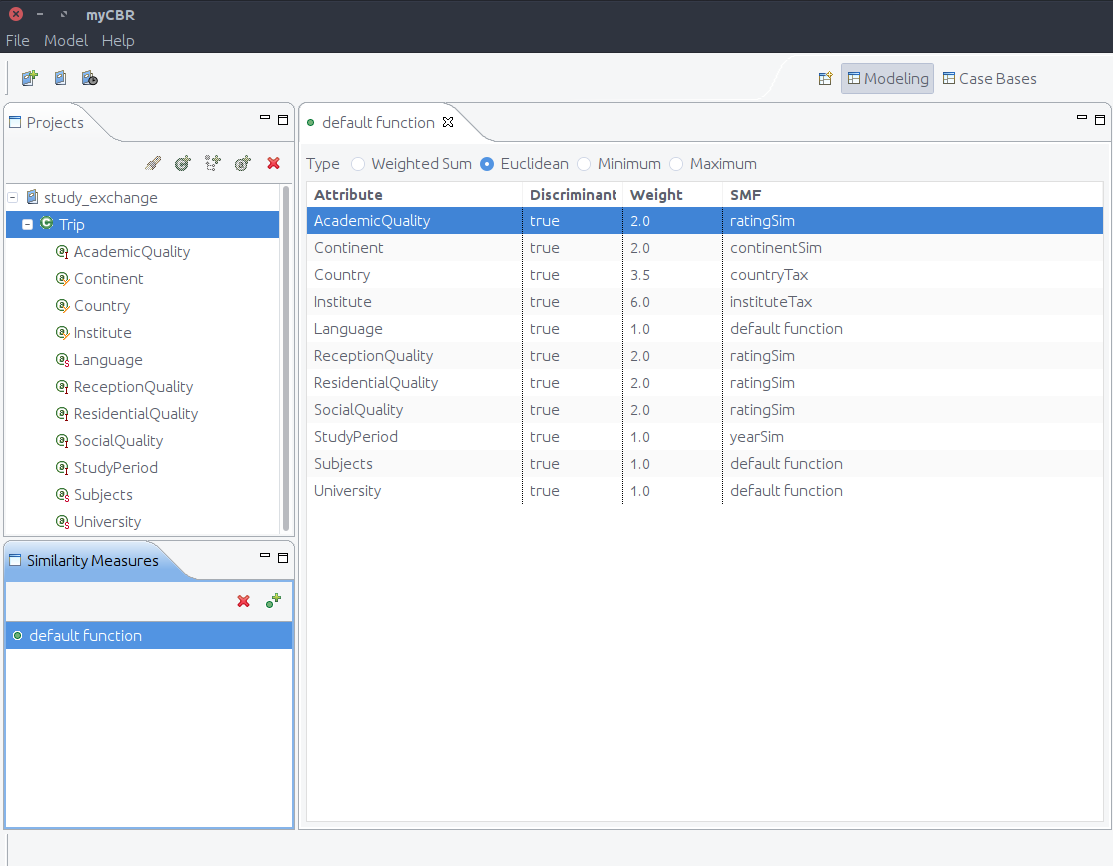
\includegraphics[width=1\textwidth]{fig/cbr_model.png}
    \caption{The similarity measure overview in the MyCBR Workbench}
\end{figure}

A Java project was creatd with the MyCBR SDK. This project imports all the parsed cases as a CSV file, and the CBR project created with the MyCBR Workbench. A Java Spring server was implemented to serve the application, with a REST framework to receive requets from Utsida, and serve back a list of the most similar cases to the query. Finally, Maven was used to compile a JAR file which runs the CBRS. 

\begin{figure}[h]
    \label{fig:retrieval_process_diagram}
    \centering
    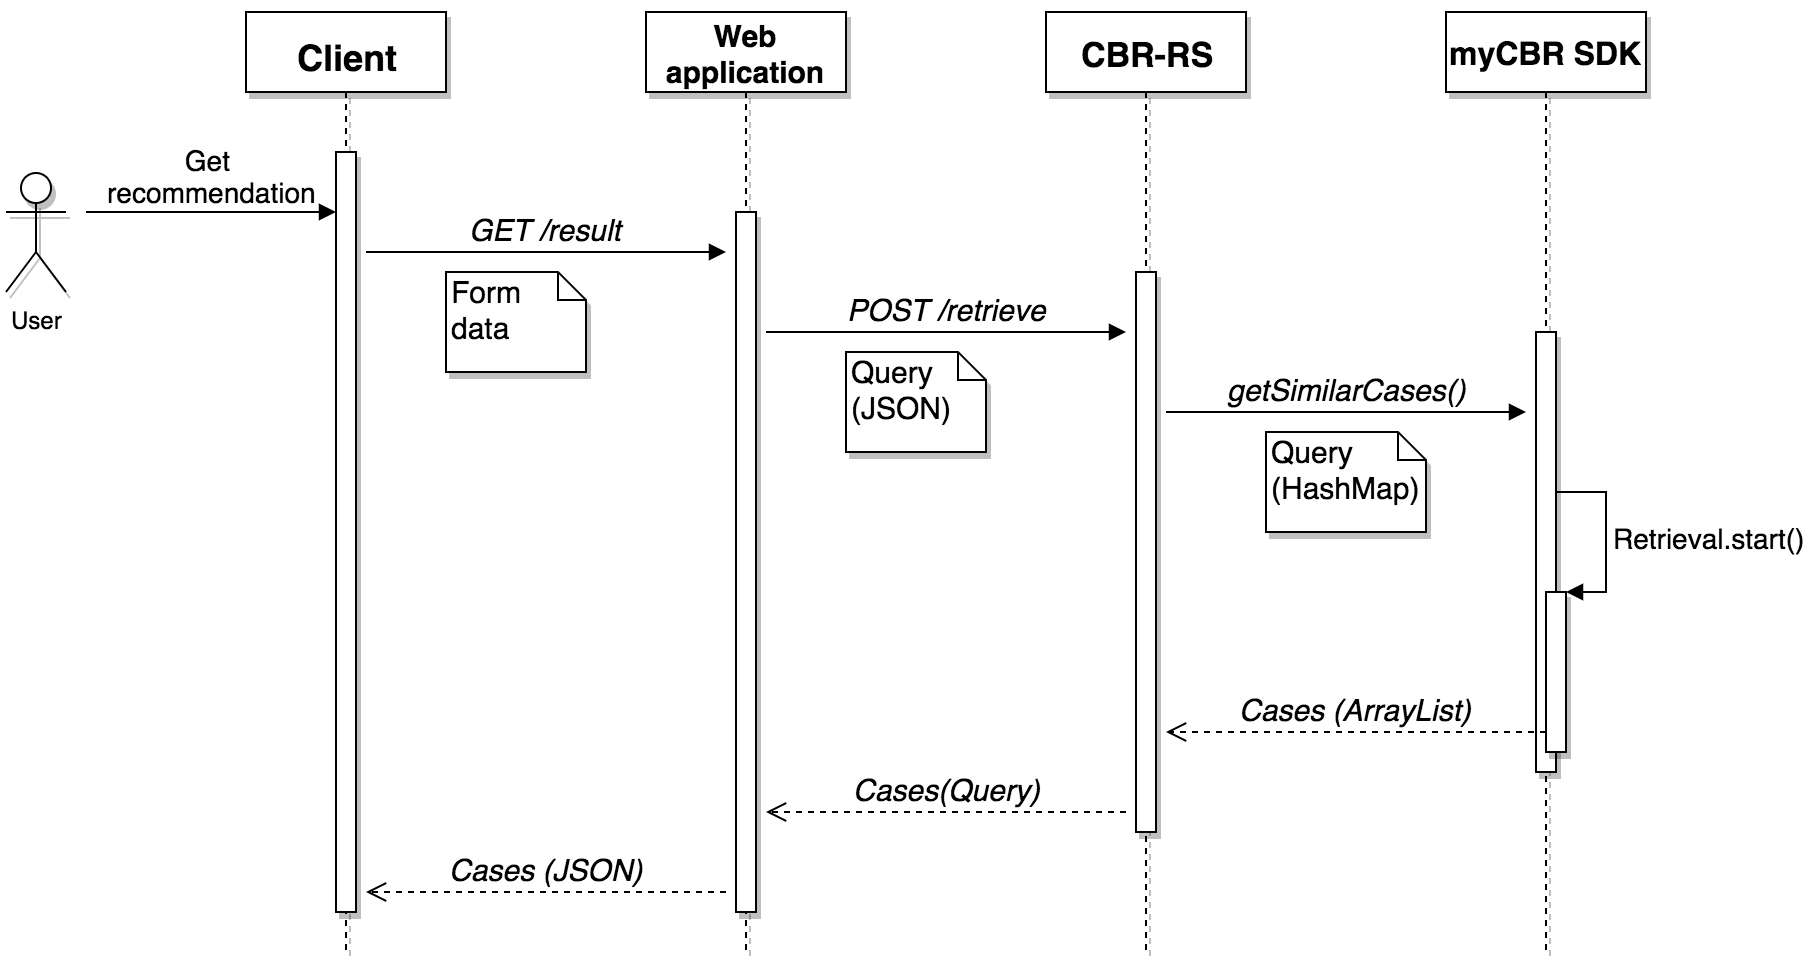
\includegraphics[width=1\textwidth]{fig/RetrievalProcessDiagram.png}
    \caption{Sequence diagram which shows how the initial user input is handled before returning as similar cases}
\end{figure}

It is important to note that this process only performs the first step of the CBR-cycle: Retrieval. It returns a set of the most similar cases to a query from Utsida. This makes the system more in line with a Case-Based Recommender System, than a standard CBRS. 

\begin{displayquote}\enquote{
In principle, recommendations need also a query. This query is, however, not asking
for a specific product. It is, rather, in the form of a more general wish. The wish may
not even be formulated explicitly by the customer. If there is a user profile, one may
generate or construct a wish that the customer is likely to have.
The answer or solution to the query problem is an item or a set of items that the
customer may want. This requires knowledge about customer’s preferences.\cite{richter2013case}
}\end{displayquote}

Similar to this definition, the query which the CBR module recieves is a \emph{wish} from a student, containing their most desired attributes, combined with information they have stated in their profile, and it returns not one, but a list of recommendations, so that the user can browse these freely, and produce a choice which may be a combination of several of the recommendations.


\section{Tools and frameworks}
When developing Utsida's web application, several tools and packages was used to simplify the development process and to acquire functionality which would not be feasible to develop from scratch. Django, see section \ref{sec:django}, was chosen as the main web framework.

To enforce a responsive and aesthetic design, Bootstrap 3\footnote{http://getbootstrap.com/} was used as a front-end CSS framework. jQuery\footnote{https://jquery.com/} was used as a front-end javascript framework to simplify HTTP requests, which this system largely relies on both internally in the web application and between the web application and the CBRS back-end. A collection of packages for the Python language was also used. These include Fuzzywuzzy\footnote{https://pypi.python.org/pypi/fuzzywuzzy}: a packages which handles apprximate string matching, requests\footnote{http://docs.python-requests.org/en/master/}: a package for writing HTTP requests from Python, and python-social-auth\footnote{https://python-social-auth.readthedocs.io/en/latest/} combined with dataporten-auth\footnote{https://pypi.python.org/pypi/dataporten-auth/0.1} to enable using authentication methods such as Feide, the authentication service used at NTNU.

\subsection{Django}\label{sec:django}
 Django\cite{djangodocs}, a web framework using the Python programming language, was chosen as the web framework to be used for Utsida. Django is maintained by the \enquote{Django Software Foundation} (DSF). The DSF calls it an \emph{MTV} framework, meaning \emph{Model, Template, View}, which in practice functions as a \emph{MVC} pattern. Django includes many built-in features such as a SQLite database, a predefined directory structure, controllers to handle communication between the different components, and several others. Another important feature is Django's built-in security packages, which handles important security risks such as Cross-Site Request Forgery, authorization and Cross-site scripting. Django also includes an administrator panel, which enabled simple management of database models with an intuitive interface. In conclusion Django offered a complete package which reduced the time used on structural difficulties and made time for more focus on methods, usability and design choices which ultimately is the reason for choosing it as the main framework.


 
\section{Design \& Usability}
The design in terms of both functionality and aesthetics was an integral part of the development of Utsida's web application. Questionnaires was used as the main data collection method to gather data on how a the system performed in terms of motivational effect as well as evaluation of the validity of the system's recommendations. This was all conducted in a remote manner, which removes the option for the authors to help the test subjects with eventual issues. Therefore, the system had to be designed in a way which would produce as little issues and hardships for the users as possible, to make sure they understood how to use it, and thus were able to truly evaluate it.

The mindset with the Design of Utsida is inspired by the \emph{User Centered System Design}-perspective, proposed by Norman D. A. \& Draper S. W (1986)\cite{norman1986user}. Real potential users of the system was included throughout the development process, either by small hallway tests, interviews, or usability tests. These tests let the users try out the system on their own, followed by questions like \enquote{How would you expect this functionality to work?}, \enquote{Was it easy to navigate the system?}, \enquote{Was it intuitive to understand how that functionality works?}. The design of Utsida is supposed to put the user in the center, and in control. Several measures was implemented to strive for this goal including:

\begin{itemize}
    \item Personalized items: Buttons and links to parts of the application which contains information and data which the user can save, change, and feel an ovnership towards are prefixed with the word \emph{My}. For example, \emph{My courses, My profile, my applications.}
    \item Inline help text: Areas of the application which may need extra information to understand properly contain hover able help text bubbles, for those who need it.
    \item Streamlined process: The main process, and common use flow is demonstrated as a numerated process, to guide the user.
\end{itemize}

\begin{figure}[h]
    \centering
    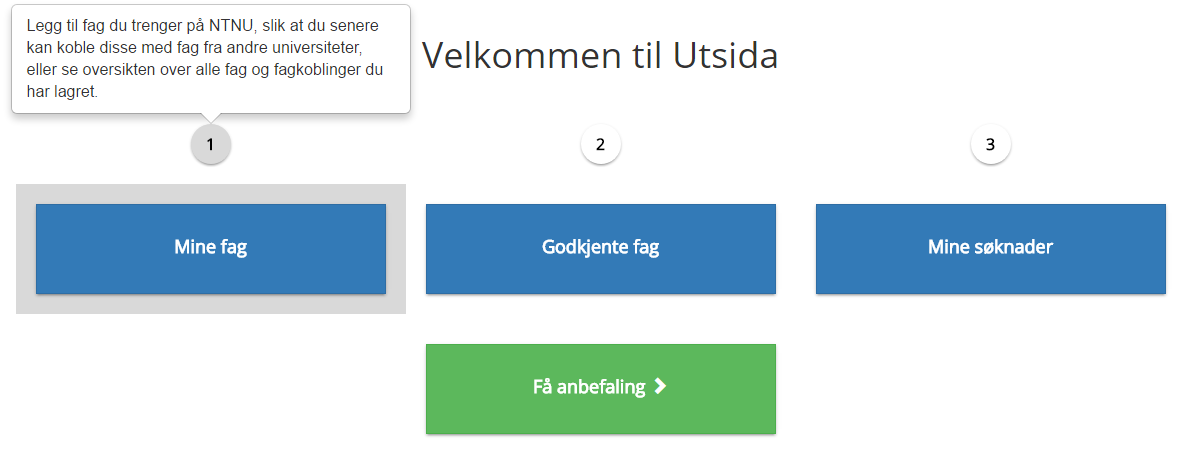
\includegraphics[width=1\textwidth]{fig/utsida_screenshots/steps.png}
    \caption{The index page of Utsida's web application}
    \label{fig:utsida_index}
\end{figure}

See Appendix \ref{app:screen_shots} for screenshots of Utsida's different views and functionalities.

\subsection{Usability Testing}
Each of the two usability test sessions during the development of Utsida produced three System Usability Scale (SUS)-schemas to measure the usability of the system. These were considered in additional to any direct feedback received after each test, as it was ideal to see and increase in these scores during the development. The first session of usability testing yielded the following SUS-scores (1-100): 67.5, 87.5 and 70, while the second session yielded as follows: 92.5, 95 and 97.5. The latter score suggested that the system was in an acceptable state to perform the final survey after the second session of usability testing.

\section{Test Environment}
To be able to perform offline usability testing and larger scale online tests the application was hosted on a virtual server provided by Department of Computer Science at NTNU. The virtual server was running Ubuntu 16.04, a debian based linux operating system. The provided domain for the application was utsida.idi.ntnu.no.

The specific HTTP web server used was Apache2, and it was configured with HTTPS to enable secure and encrypted user sessions. To reduce the effort of running online usability tests and enable users to log in through their university account a service platform using UNINETT's federated authentication service (FEIDE) was implemented. The service platform "Dataporten"\cite{dataporten} provided by UNINETT enables quick access to important user data and makes possible application users able to log in without registering a user. 

Error reporting through email was configured on the server so that alerts were given in case of possible downtime or server errors. Error reporting made it possible to quickly resolve potential bugs or errors on the application and ensure higher user satisfaction when running user tests. Tracking user behaviour and statistics could be useful in the final data analysis. Google Analytics was therefore used to increase the understanding of user behaviour. Through Google Analytics it is possible to see a large set of data on the user behaviour. The most important ones used in this project were number of users, average session time, device type and activity flow.  

\cleardoublepage